\chapter*{Wprowadzenie}
\addcontentsline{toc}{chapter}{Wprowadzenie}
\begin{figure}
 \centering
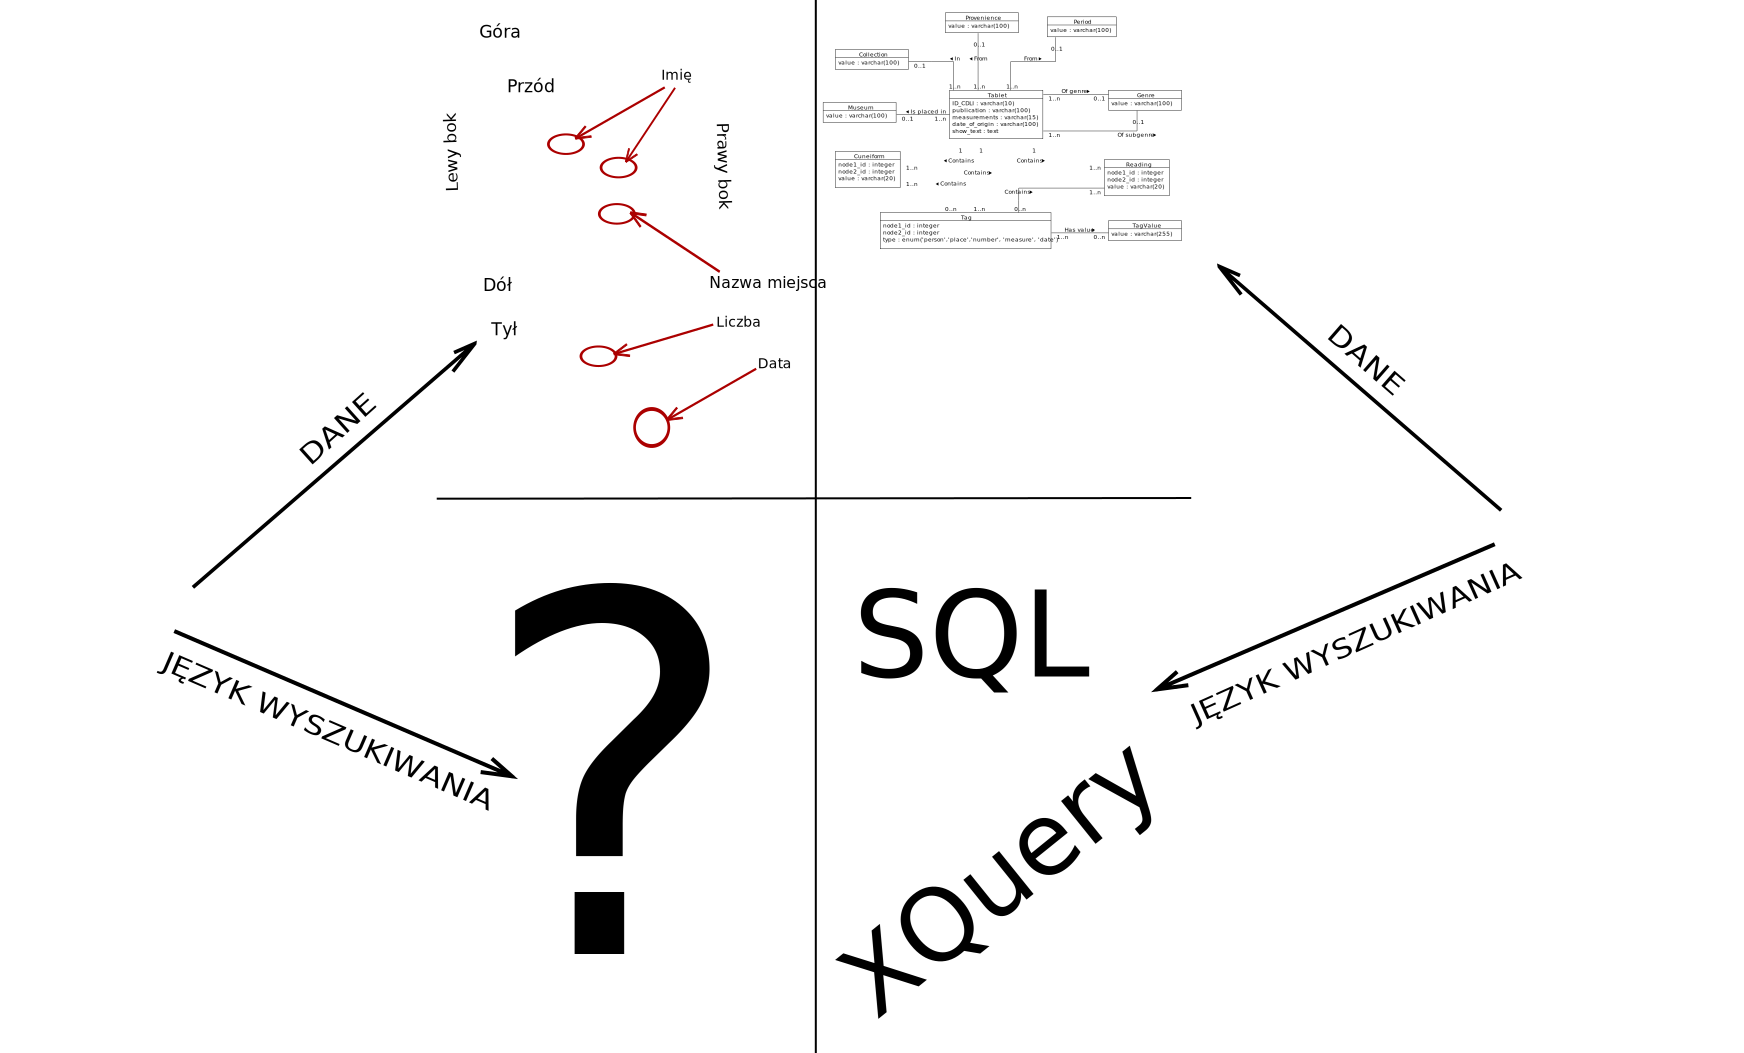
\includegraphics[width=400px]{./diagramy/poco.pdf}
 \caption{Miejsce TQL w świecie}
\end{figure}


\ \ \ \ Sumerolodzy posiadają bazę danych składającą się z prawie 225 tys. tabliczek sumeryjskich w wersji elektronicznej. 
Potrzebują prostego i intuicyjnego języka służącego do ich wyszukiwania, który jak najmniej będzie ograniczał siłę wyrazu,
 a jego wykorzystanie będzie powodowało jak najmniejszy narzut czasowy.

Istnieją też inne grupy ludzi potrzebujące podobnego języka (np. językoznawcy). 
Większość programów ułatwiających tworzenie zapytań jest skomplikowana, daje ograniczone możliwości lub jest przystosowana głównie do przetwarzania danych liczbowych. Tablets Query Language rozwiązuje te problemy: jest prosty i intuicyjny, przystosowany głównie do tekstów, minimalnie zmniejsza siłę wyrazu oraz łatwo go rozbudowywać. 

%Język TQL jest nakładką na inne języki (m.in. SQL). 
TQL jest jednym z języków dziedzinowych (Domain Specific Languages, DSL). 
W związku z tym dla każdego sposobu reprezentacji danych należy skonstruować translator, 
którego zadaniem będzie przetłumaczenie zapytania. 
% Dla każdego z nich, w zależności od reprezentacji danych, należy skonstruować translator, 
% którego zadaniem będzie przetłumaczenie zapytania. 
W ramach niniejszej pracy przedstawione zostaną dwa przykładowe translatory.
